\subsection{Techniki prezentacji danych w aplikacjach webowych}

\subsubsection{Wykresy jednej zmiennej}

Są to metody, które pozwalają na wizualizację jednej cechy (dwóch licząc uwzględnienie klasy na wykresie np. przez kolor). Dzięki nim możemy obejrzeć rozkład cechy, wartości średnie, odchylenie standardowe itp.. Zaliczamy do nich m.in. wykresy pudełkowe oraz histogramy. Histogramy są narzędziem, dzięki któremu możemy graficznie odtworzyć rozkład danej cechy. Poza tym pozwalają one również dostrzec rozpiętość, skośność oraz szum danych. Często podczas tworzenia histogramów wprowadza się podział na klasy.

\begin{figure}[H]
	\centering
	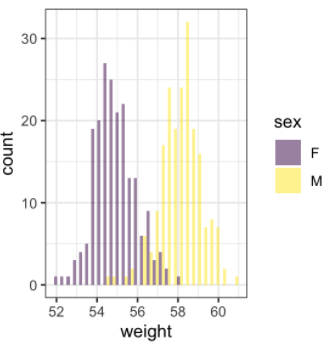
\includegraphics[width=0.3\linewidth]{S5.png}
\end{figure}

\subsubsection{Rzut na dwie współrzędne}

Do tej grupy zaliczamy metody, które pozwalają pokazać jednocześnie dwie współrzędne. Techniki te umożliwiają odkrycie związków między cechami (np. korelacja). Wykresy rozproszone (ang. scatterplot) są podstawowym narzędziem, które rzutuje dane na dwie współrzędne. Ich analiza powinna odbywać się pod kątem odkrycia korelacji między poszczególnymi cechami oraz klasteryzacji danych. Wykresy rozproszone są tworzone poprzez zaznaczanie kolejnych punktów danych w przestrzeni dwuwymiarowej. Wartość współrzędnej X odnosi się do pierwszej cechy, a Y do drugiej. Często mamy do czynienia z danymi podzielonymi na klasy

\begin{figure}[H]
	\centering
	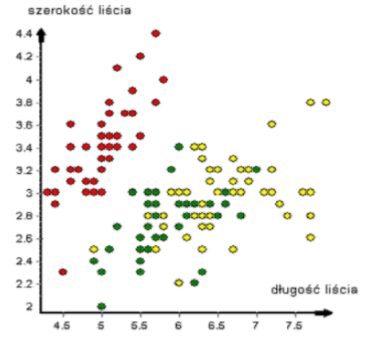
\includegraphics[width=0.4\linewidth]{S5_1.png}
\end{figure}

Drugą metodą pozwalającą jednoczesne pokazanie dwóch cech są, wcześniej wymienione, histogramy dwuwymiarowe

\begin{figure}[H]
	\centering
	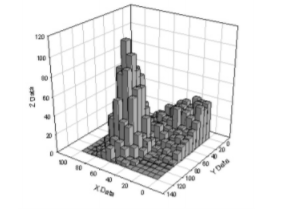
\includegraphics[width=0.4\linewidth]{S5_2.png}
\end{figure}

\subsubsection{Metody używające koloru i odcieni}

Jest to kolejny pomysł na wizualizację danych, wykorzystujący naturalne ludzkie zdolności rozróżniania kolorów (dotyczy ludzi nie cierpiących na choroby takie jak daltonizm). Do metod tych należą prostokąty heatmap’y, gdzie kolor odpowiada wartości cechy w zależności od dwóch pozostałych współrzędnych. \\

Heatmap’y są także wykorzystywane przy dużych zbiorach danych, np. do macierzy konfuzji przy sprawdzaniu modeli sztucznej inteligencji. Bardziej niż na dokładnej wartości, zależy nam aby sprawdzić czy przewidywane klasy odpowiadają rzeczywistym, i na pierwszy rzut oka da się dostrzeć w jakich obszarach/jakie klasy błędnie interpretuje np. sieć neuronowa

\begin{figure}[H]
	\centering
	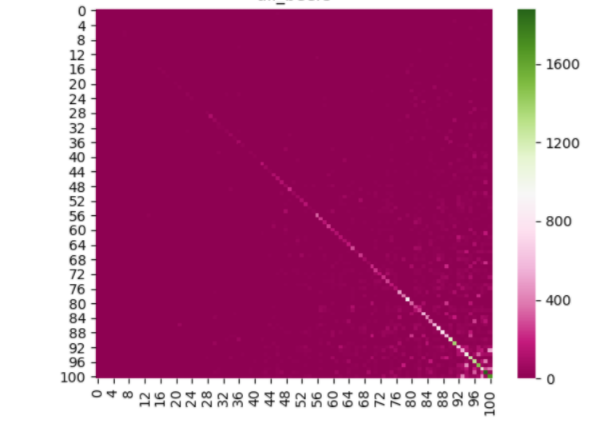
\includegraphics[width=0.4\linewidth]{S5_3.png}
\end{figure}

\subsubsection{Metody korzystające z osi gwiazdowych (radarowych)}

Ta grupa składa się tylko z jednej metody czyli wykresów gwiazdowych (ang. star plot, radar plot). Technika pozwala na zaprezentowanie danych wielowymiarowych z dowolną ilością zmiennych. Każdy wektor cech jest reprezentowany przez wykres, przypominający gwiazdę, w którym każdy promień przedstawia jedną zmienną

\begin{figure}[H]
	\centering
	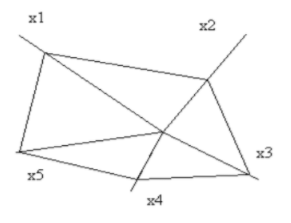
\includegraphics[width=0.3\linewidth]{S5_4.png}
\end{figure}